\documentclass[10pt]{article}
\usepackage[utf8]{inputenc}
\usepackage[T1]{fontenc}
\usepackage{graphicx}
\usepackage{tikz}
\usetikzlibrary{arrows}
\usepackage[export]{adjustbox}
\usepackage{amsmath}
\usepackage{amsfonts}
\usepackage{amssymb}
\usepackage[version=4]{mhchem}
\usepackage{stmaryrd}
\usepackage{tikz}


\title{Problem set 12}


\author{by Maksim Al Dandan}

\begin{document}
\maketitle

\section*{Week 12. Problem set}
\section{Task 1}
\subsection{Statement}

Run Prim-Jarník algorithm [Cormen, §21.2] on the following graph, starting at vertex $C$. Assuming that the algorithm is using Binary heap implementation [Cormen, $\S 6$] of a priority queue, show the state of the Binary heap after each iteration of the algorithm (i.e. after adding each new vertex to the MST). The graph contains 8 vertices, which means that your solution must provide 8 states of the Binary heap. Each heap state must be represented as an array. No justification is required.

\begin{center}
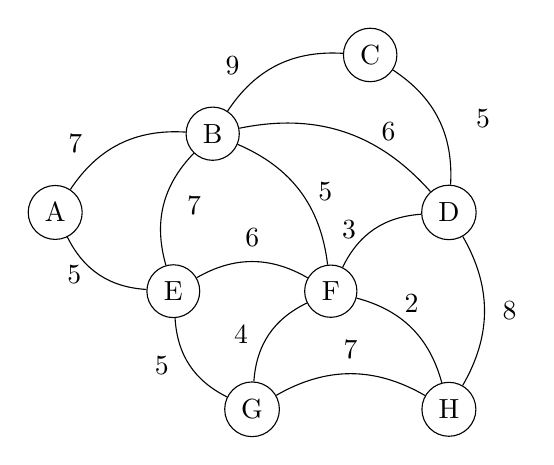
\begin{tikzpicture}

\tikzset{vertex/.style = {shape=circle,draw,minimum size=1.5em}}
\tikzset{edge/.style = {-,> = latex',thick}}
% vertices
\node[vertex] (a) at  (0,0)   {A};
\node[vertex] (b) at  (2,1)   {B};
\node[vertex] (c) at  (4,2)   {C};
\node[vertex] (d) at  (5,0)   {D};
\node[vertex] (e) at  (1.5,-1)  {E};
\node[vertex] (f) at  (3.5,-1)  {F};
\node[vertex] (g) at  (2.5,-2.5) {G};
\node[vertex] (h) at  (5,-2.5)  {H};

%edges

\draw[] (b) to[bend right] node [midway, left= 10pt] {7} (a);
\draw[] (b) to[bend left] node [midway, left= 10pt] {9}(c);
\draw[] (b) to[bend left] node [midway, right= 10pt] {6} (d);
\draw[] (c) to[bend left] node [midway, right= 10pt] {5} (d);
\draw[] (b) to[bend left] node [midway, right= 3pt] {5} (f);
\draw[] (d) to[bend left] node [midway, right = 3pt] {8} (h);
\draw[] (b) to[bend right] node [midway, right= 5pt] {7} (e);
\draw[] (a) to[bend right] node [midway, left= 3pt] {5} (e);
\draw[] (f) to[bend left] node [midway, left= 3pt] {3} (d);
\draw[] (f) to[bend left] node [midway,  above=2pt] {2} (h);
\draw[] (f) to[bend right] node [midway,  above=2pt] {6} (e);
\draw[] (g) to[bend left] node [midway, left= 4pt] {5} (e);
\draw[] (g) to[bend left] node [midway, left= 4pt] {4} (f);
\draw[] (g) to[bend left] node [midway, above = 2pt] {7} (h);
    


\end{tikzpicture}
\end{center}

\subsection{Solution}

\begin{center}
\begin{tabular}{|c|c|c|c|c|c|c|c|c|}
\hline
\textbf{Number} & \textbf{Vertices} & \textbf{Edges} & \textbf{Weights} \\
\hline
1. & - & - & - \\
\hline
2. & B & CB & 9 \\
\hline
3. & B & DB & 6 \\
\hline
& H & DH & 8 \\
\hline
4. & B & FB & 5 \\
\hline
& G & FG & 4 \\
\hline
& E & FE & 6 \\
\hline
5. & E & GE & 5 \\
\hline
6. & A & BA & 7 \\
\hline
7. & A & EA & 5 \\
\hline
8. & - & - & - \\
\hline
\end{tabular}
\end{center}

\section{Task 2}
\subsection{Statement}

Suppose that all edge weights in a graph are integers in the range from 1 to $|V|$. How fast can you make Kruskal's algorithm run by modifying it somehow? What if the edge weights are integers in the range from 1 to $W$ for some constant $W$? Justify your answer in at most two paragraphs.

\subsection{Solution}

If all edge weights in a graph are integers in the range from 1 to $|V|$, we can use a linear time sorting algorithm such as counting sort instead of a comparison-based sorting algorithm. This would make the sorting step of Kruskal's algorithm run in $O(V + E)$ time, and since the disjoint-set operations run in nearly constant time, the overall time complexity of the algorithm would be $O(V + E)$.

If the edge weights are integers in the range from 1 to $W$ for some constant $W$, we can still use counting sort or radix sort to sort the edges in linear time. However, if $W$ is significantly larger than $|V|$ and $|E|$, the time complexity of the sorting step could be dominated by $W$. In this case, the overall time complexity of the algorithm would be $O(W + V + E)$.

\section*{References}
[Cormen] T. H. Cormen, C. E. Leiserson, R. L. Rivest and C. Stein. Introduction to Algorithms, Fourth Edition. The MIT Press 2022


\end{document}